\documentclass[tikz,border=5pt]{standalone}
\usepackage{amsmath}
\definecolor{curveblue}{HTML}{245C86}
\begin{document}
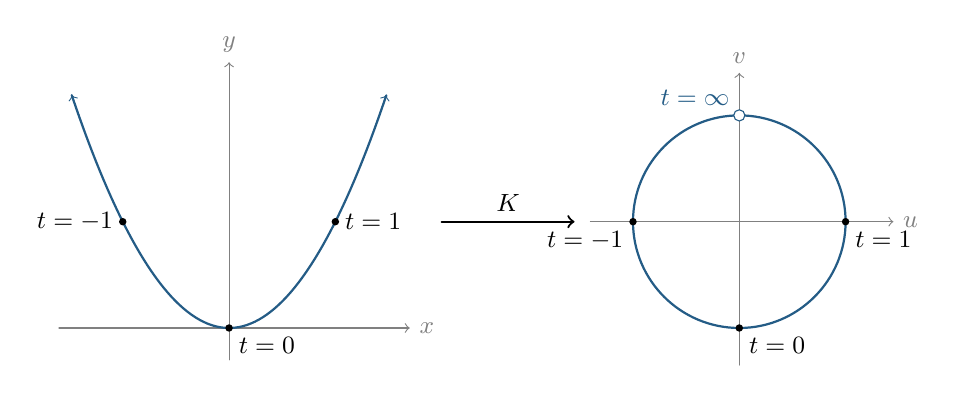
\begin{tikzpicture}[scale=1.35,font=\small,line cap=round]
\begin{scope}[xshift=-2.8cm]
\draw[gray,->](-1.6,0)--(1.7,0)node[right]{$x$};
\draw[gray,->](0,-.3)--(0,2.5)node[above]{$y$};
\draw[curveblue,thick,domain=-1.48:1.48,samples=80]plot(\x,{\x*\x});
\fill(-1,1)circle(1pt)node[left]{$t=-1$};\fill(1,1)circle(1pt)node[right]{$t=1$};
\fill(0,0)circle(1pt)node[below right]{$t=0$};
\draw[curveblue,->](-1.37,1.88)--(-1.48,2.19);
\draw[curveblue,->](1.37,1.88)--(1.48,2.19);
\end{scope}
\draw[->,thick](-.8,1)--(.45,1)node[midway,above]{$K$};
\begin{scope}[xshift=2cm,yshift=1cm]
\draw[gray,->](-1.4,0)--(1.45,0)node[right]{$u$};
\draw[gray,->](0,-1.35)--(0,1.4)node[above]{$v$};
\draw[curveblue,thick](0,0)circle(1);
\fill(-1,0)circle(1pt)node[below left]{$t=-1$};
\fill(1,0)circle(1pt)node[below right]{$t=1$};
\fill(0,-1)circle(1pt)node[below right]{$t=0$};
\draw[curveblue,fill=white](0,1)circle(1.5pt)node[above left]{$t=\infty$};
\end{scope}
\end{tikzpicture}
\end{document}
